\documentclass[border=0pt]{standalone}
\newcommand{\revlamina}{4}
\providecommand{\revlamina}{1}
% Preámbulo común de las láminas FV (A3 horizontal, 420 x 297 mm)
\usepackage[T1]{fontenc}
\usepackage[utf8]{inputenc}
\usepackage[spanish,es-nodecimaldot]{babel}
\usepackage[scaled=0.92]{helvet}
\renewcommand{\familydefault}{\sfdefault}
\usepackage{tikz}
\usetikzlibrary{arrows.meta,patterns,calc,babel,positioning}
\usepackage{siunitx}
\sisetup{output-decimal-marker={,},mode=text}
\DeclareSIUnit\kWp{kWp}
\DeclareSIUnit\ohm{\ensuremath{\Omega}}

\definecolor{inv1}{RGB}{37,99,180}
\definecolor{inv2}{RGB}{22,128,84}
\definecolor{nfpa}{RGB}{200,30,30}
\definecolor{viento}{RGB}{40,70,200}
\definecolor{sombra}{RGB}{230,130,0}
\definecolor{losa}{RGB}{120,190,200}
\definecolor{dc}{RGB}{225,95,0}
\definecolor{exist}{RGB}{110,110,110}
\definecolor{nuevo}{RGB}{190,20,20}

% Marcador de referencia numerada
\newcommand{\refm}[2]{\node[circle,draw=black,fill=white,line width=0.35pt,inner sep=0pt,minimum size=3.4mm,font=\fontsize{5.5}{6}\selectfont\bfseries] at #1 {#2};}

% Cajetín: \cajetin{lamina}{titulo}{contenido}{escala}{hoja}
\newcommand{\cajetin}[5]{%
  \draw[line width=0.6pt] (250,10) rectangle (410,58);
  \draw[line width=0.3pt] (250,46) -- (410,46);
  \draw[line width=0.3pt] (250,34) -- (410,34);
  \draw[line width=0.3pt] (250,22) -- (410,22);
  \draw[line width=0.3pt] (370,10) -- (370,34);
  \draw[line width=0.3pt] (330,10) -- (330,22);
  \node[anchor=north west,font=\fontsize{6}{7}\selectfont,align=left] at (251.5,57) {\textbf{Instituto Tecnológico de Costa Rica} -- EL-4601 Normalización Técnica para Electrónica\\Proyecto No.~2: Diseño normativo de una instalación solar fotovoltaica};
  \node[anchor=north west,font=\fontsize{6}{7}\selectfont,align=left] at (251.5,45) {\textbf{Proyecto:} Sistema FV 20,88~kWp -- Edificio Centro Académico de Alajuela (TEC)\\\textbf{Propietario:} Universidad Técnica Nacional -- Catastro A-652521-2000};
  \node[anchor=north west,font=\fontsize{6.5}{7.5}\selectfont,align=left,text width=115mm] at (251.5,33) {\textbf{Contenido:} #2\\#3};
  \node[anchor=north west,font=\fontsize{5.5}{6.5}\selectfont,align=left] at (371.5,33) {\textbf{Lámina}};
  \node[font=\fontsize{16}{18}\selectfont\bfseries] at (390,25.5) {#1};
  \node[anchor=north west,font=\fontsize{5.5}{6.5}\selectfont,align=left] at (251.5,21) {\textbf{Elaboró:} Grupo de trabajo EL-4601\\\textbf{Revisó:} \rule{25mm}{0.2pt}\\\textbf{Fecha:} 7/10/2026 \quad \textbf{Rev.:} \revlamina};
  \node[anchor=north west,font=\fontsize{5.5}{6.5}\selectfont,align=left] at (331.5,21) {\textbf{Escala (A3):}\\#4};
  \node[anchor=north west,font=\fontsize{5.5}{6.5}\selectfont,align=left] at (371.5,21) {\textbf{Hoja:}\\#5};
}
% Marco de la lámina
\newcommand{\marco}{%
  \draw[line width=0.2pt,white] (0,0) rectangle (420,297);
  \draw[line width=0.8pt] (10,10) rectangle (410,287);
}

\begin{document}
\begin{tikzpicture}[x=1mm,y=1mm]
\marco
\node[anchor=north west,inner sep=0pt] at (15.00,280.00) {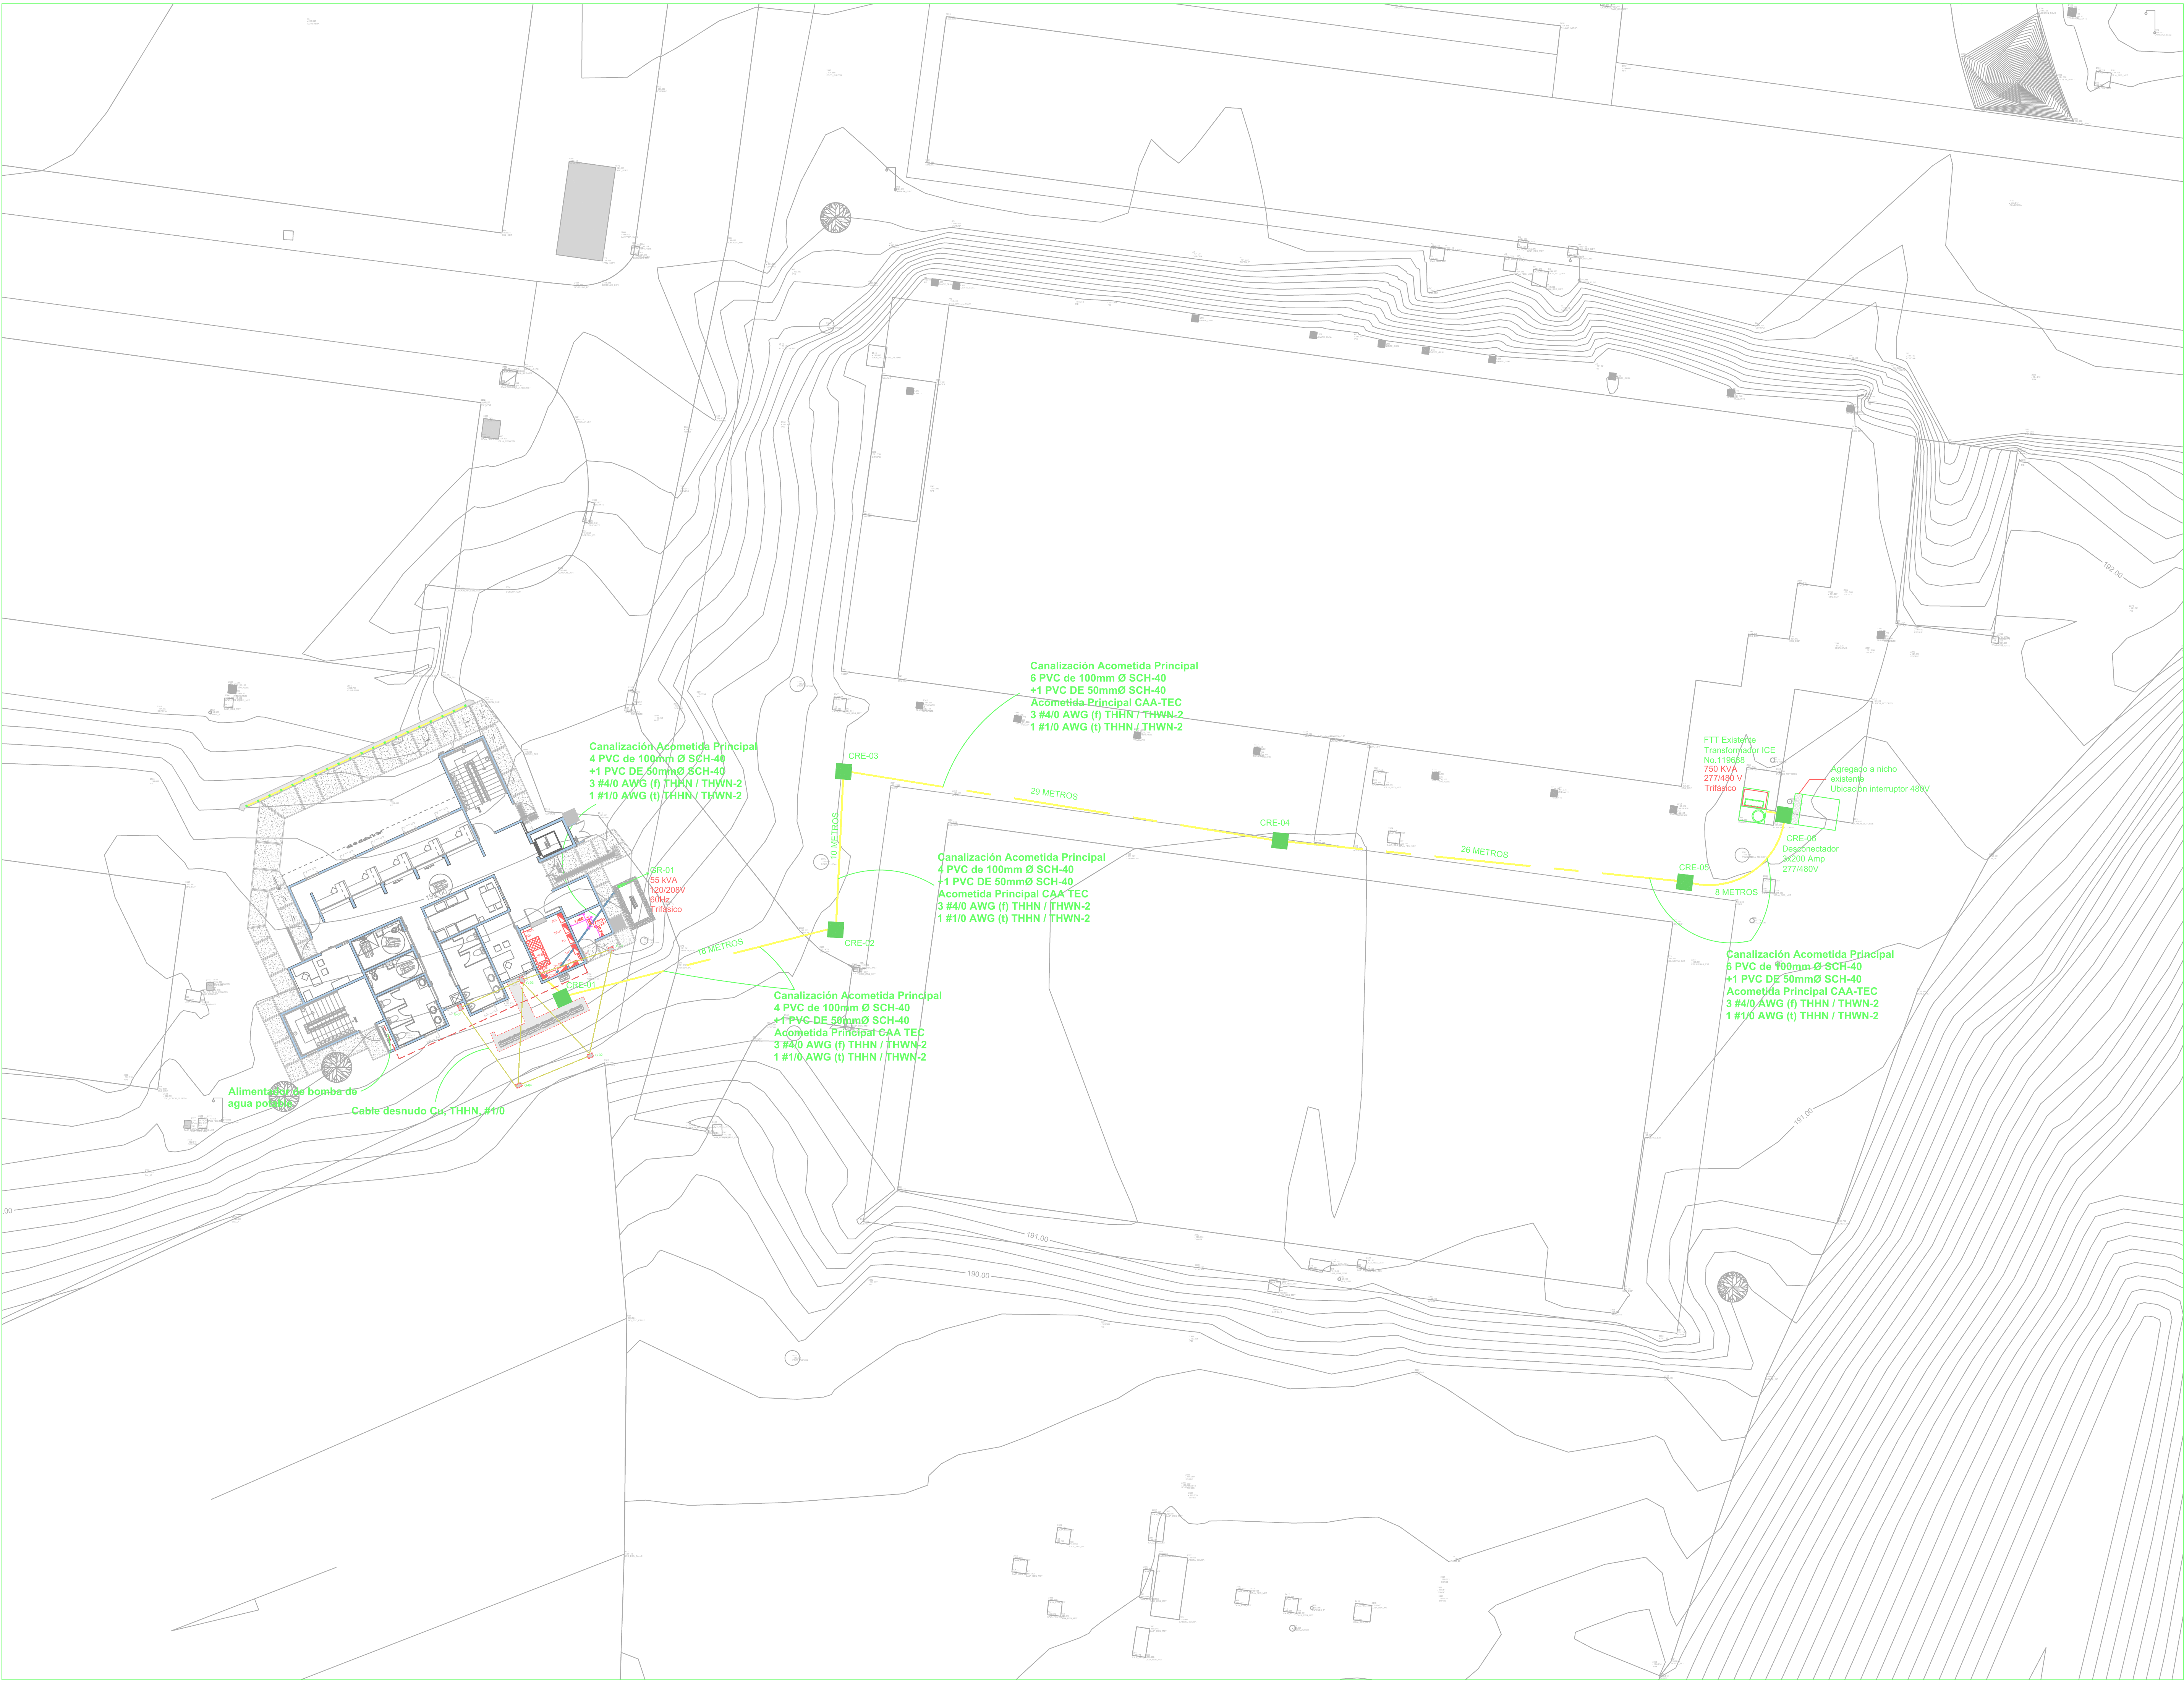
\includegraphics[width=225mm]{fv00_base.png}};
\draw[line width=0.4pt] (15.00,280.00) rectangle ++(225,-173.2);
\begin{scope}[shift={(226.00,122.00)},rotate=-10]
\filldraw[fill=white,draw=black,line width=0.4pt] (0,0) circle (6);
\fill[black] (0,5.2) -- (-2.2,-3.8) -- (0,-2.2) -- cycle; \draw[black,line width=0.4pt,fill=white] (0,5.2) -- (2.2,-3.8) -- (0,-2.2) -- cycle;
\node[font=\fontsize{8}{9}\selectfont\bfseries] at (0,8.2) {N};
\end{scope}
\draw[inv1,line width=0.4pt] (61.36,187.94) -- (40.00,268.00);
\filldraw[inv1,draw=black,line width=0.3pt] (61.36,187.94) circle (1.1);
\node[anchor=west,draw=inv1,fill=white,line width=0.4pt,inner sep=1.2pt,font=\fontsize{6}{7}\selectfont] at (40.00,268.00) {\textbf{1} \ Edificio CAA-TEC: arreglo FV de 20,88 kWp en la cubierta (FV-01)};
\draw[nuevo,line width=0.4pt] (72.18,182.70) -- (40.00,128.00);
\filldraw[nuevo,draw=black,line width=0.3pt] (72.18,182.70) circle (1.1);
\node[anchor=west,draw=nuevo,fill=white,line width=0.4pt,inner sep=1.2pt,font=\fontsize{6}{7}\selectfont] at (40.00,128.00) {\textbf{2} \ Cuarto eléctrico (TS-01, ATS, TP) y equipos FV en la fachada sur (FV-02)};
\draw[exist,line width=0.4pt] (83.11,188.38) -- (115.00,250.00);
\filldraw[exist,draw=black,line width=0.3pt] (83.11,188.38) circle (1.1);
\node[anchor=west,draw=exist,fill=white,line width=0.4pt,inner sep=1.2pt,font=\fontsize{6}{7}\selectfont] at (115.00,250.00) {\textbf{3} \ Generador Kohler existente (E07: J100U-IV, 100 kW)};
\draw[inv2,line width=0.4pt] (72.94,174.72) -- (40.00,118.00);
\filldraw[inv2,draw=black,line width=0.3pt] (72.94,174.72) circle (1.1);
\node[anchor=west,draw=inv2,fill=white,line width=0.4pt,inner sep=1.2pt,font=\fontsize{6}{7}\selectfont] at (40.00,118.00) {\textbf{4} \ Malla de tierra existente, registros G-01 a G-05 ($\le$ 5 $\Omega$)};
\draw[exist,line width=0.4pt] (73.60,178.54) -- (120.00,138.00);
\filldraw[exist,draw=black,line width=0.3pt] (73.60,178.54) circle (1.1);
\node[anchor=west,draw=exist,fill=white,line width=0.4pt,inner sep=1.2pt,font=\fontsize{6}{7}\selectfont] at (120.00,138.00) {\textbf{5} \ CRE-01: llegada de la acometida de 480 V};
\draw[dc,line width=0.4pt] (144.77,195.60) -- (120.00,155.00);
\filldraw[dc,draw=black,line width=0.3pt] (144.77,195.60) circle (1.1);
\node[anchor=west,draw=dc,fill=white,line width=0.4pt,inner sep=1.2pt,font=\fontsize{6}{7}\selectfont] at (120.00,155.00) {\textbf{6} \ Acometida 480 V: 1\#4/0 Cu por fase, $\approx$100 m, en ductos PVC};
\draw[nuevo,line width=0.4pt] (195.39,197.24) -- (150.00,238.00);
\filldraw[nuevo,draw=black,line width=0.3pt] (195.39,197.24) circle (1.1);
\node[anchor=west,draw=nuevo,fill=white,line width=0.4pt,inner sep=1.2pt,font=\fontsize{6}{7}\selectfont] at (150.00,238.00) {\textbf{7} \ Transformador ICE N.\textsuperscript{o} 119688, 750 kVA, 34,5 kV/480Y/277 V};
\draw[exist,line width=0.4pt] (202.83,195.60) -- (150.00,228.00);
\filldraw[exist,draw=black,line width=0.3pt] (202.83,195.60) circle (1.1);
\node[anchor=west,draw=exist,fill=white,line width=0.4pt,inner sep=1.2pt,font=\fontsize{6}{7}\selectfont] at (150.00,228.00) {\textbf{8} \ Nicho: interruptor 200 A/3P 480 V y medición ICE (supuesta)};
\node[anchor=north west,font=\fontsize{10}{12}\selectfont\bfseries] at (15,100) {PLANO GENERAL DE UBICACIÓN -- CAMPUS SEDE CENTRAL UTN, VILLA BONITA DE ALAJUELA};
\node[anchor=north west,font=\fontsize{7}{8}\selectfont,align=left] at (15,94) {Base: lámina E01 ``Planta de distribución de canalización y red eléctrica'' (as-built TEC, escala original 1:200), reducida sin escala exacta.\\Orientación: norte real aproximado según la flecha (nota 7). En FV-01 y FV-02 se usa el norte de proyecto (deducido de A02), girado $\approx$30° respecto al real.};
\begin{scope}[shift={(15,80)}]
\fill[black] (0.00,0) rectangle ++(15.50,1.6);
\fill[white] (15.50,0) rectangle ++(15.50,1.6);
\fill[black] (30.99,0) rectangle ++(15.50,1.6);
\fill[white] (46.49,0) rectangle ++(15.50,1.6);
\fill[black] (61.98,0) rectangle ++(15.50,1.6);
\draw[line width=0.3pt] (0,0) rectangle (77.48,1.6);
\node[font=\fontsize{5}{6}\selectfont,anchor=north] at (0.00,-0.3) {0};
\node[font=\fontsize{5}{6}\selectfont,anchor=north] at (15.50,-0.3) {10};
\node[font=\fontsize{5}{6}\selectfont,anchor=north] at (30.99,-0.3) {20};
\node[font=\fontsize{5}{6}\selectfont,anchor=north] at (46.49,-0.3) {30};
\node[font=\fontsize{5}{6}\selectfont,anchor=north] at (61.98,-0.3) {40};
\node[font=\fontsize{5}{6}\selectfont,anchor=north] at (77.48,-0.3) {50};
\node[font=\fontsize{5}{6}\selectfont,anchor=west] at (78.48,0.8) {m (aprox.)};
\end{scope}
\node[anchor=north west,font=\fontsize{9}{11}\selectfont\bfseries] at (252,284) {DATOS DEL EMPLAZAMIENTO};
\node[anchor=north west,font=\fontsize{6.2}{7.6}\selectfont] at (252,277) {%
\setlength{\tabcolsep}{2pt}\begin{tabular}{@{}p{38mm}p{112mm}@{}}
Provincia / cantón & Alajuela / Alajuela (Central)\\
Ubicación & Sede Central UTN, Villa Bonita; el TEC la ubica en Desamparados de Alajuela ($\approx$960 msnm)\\
Coordenadas & 10,0057\,°N; 84,2164\,°O (GPS de las fotografías del 5/10/2026, $\pm$10 m)\\
Propietario / catastro & Universidad Técnica Nacional; A-652521-2000; folio real 2-363445-000\\
Usuario / uso & TEC -- Centro Académico de Alajuela; académico y administrativo\\
Distribuidora & ICE; transformador de pedestal N.\textsuperscript{o} 119688, 750 kVA, 34,5 kV/480Y/277 V\\
Servicio del edificio & 480 V trifásico desde el nicho del transformador; TS-01 480$\Delta$/208Y-120 V en el cuarto eléctrico\\
Respaldo & ATS de 400 A + generador; UPS de 20 kVA para circuitos TRU\\
Sistema FV & 20,88 kWp DC / 20 kW AC; autoconsumo con inyección de excedentes (Ley 10086)\\
\end{tabular}};
\node[anchor=north west,font=\fontsize{9}{11}\selectfont\bfseries] at (252,205) {ÍNDICE DE LÁMINAS};
\node[anchor=north west,font=\fontsize{6.2}{7.6}\selectfont] at (252,198) {%
\setlength{\tabcolsep}{2pt}\begin{tabular}{@{}ll@{}}
\textbf{FV-00} & Plano general de ubicación (esta lámina)\\
\textbf{FV-01} & Planta de cubierta: distribución del arreglo, pasillos, exclusiones y ruta DC\\
\textbf{FV-02} & Planta parcial nivel 1 y elevación: inversores, tableros y desconectadores\\
\textbf{FV-03} & Diagrama unifilar completo e interconexión\\
\textbf{FV-04} & Puesta a tierra, medios de desconexión y rotulación\\
\end{tabular}};
\node[anchor=north west,font=\fontsize{9}{11}\selectfont\bfseries] at (252,160) {NOTAS};
\node[anchor=north west,font=\fontsize{6}{7.4}\selectfont,align=left,text width=152mm] at (252,154) {%
1. Las posiciones de los elementos se transcriben de E01 (as-built). La lámina no tiene escala exacta: usar las cotas de FV-01 y FV-02.\\
2. El número del transformador del ICE (119688) y su capacidad se tomaron del rótulo de E01. Se supone que el abonado del servicio es el TEC, con tarifa T-CS (sección 5.8 del documento).\\
3. El punto de interconexión FV está dentro del edificio, en el alimentador TS-01 $\rightarrow$ ATS (lado normal). No se modifica la acometida ni el equipo del ICE.\\
4. E01 rotula el generador como GR-01 de 55 kVA y E07 lo indica como Kohler J100U-IV de 100 kW. En sitio se confirmó un grupo Kohler en cabina; se adopta el dato de E07, el unifilar de diseño. Su capacidad no influye en el sistema FV, que queda del lado normal del ATS.\\
5. La imagen satelital (sección 5.1 del documento) y el registro fotográfico (Anexo D) confirman que el edificio está girado unos 30° y que la cubierta cae hacia el ENE (azimut real de unos 60°). Los árboles cercanos tienen la copa cerca de la altura del alero.\\
6. Medición del ICE: ni los planos ni el cuarto eléctrico muestran el medidor. La acometida del CAA se agregó al nicho existente del transformador (E01); se adopta como supuesto de diseño una medición indirecta (TC) en 480 V en ese nicho, que el ICE sustituye por un medidor bidireccional (FV-03).\\
7. La flecha indica el norte real aproximado ($\pm$10°), obtenido al superponer la imagen satelital (bordes de la cubierta a 60° y 150°) con el contorno del edificio en E01.};
\cajetin{FV-00}{Plano general de ubicación del sistema FV,}{acometida, transformador ICE y equipos principales}{Sin escala (base E01 1:200)}{1 de 5}
\end{tikzpicture}
\end{document}